\documentclass[times, doublespace]{simauth}

\usepackage{moreverb}
\usepackage[colorlinks,bookmarksopen,bookmarksnumbered,citecolor=red,urlcolor=red]{hyperref}
 \usepackage[numbers, square, sort&compress]{natbib}
 
 
\begin{document}
% The following line would print the thesis in 
%opening

\runninghead{EE Gabriel and MC Sachs and PB Gilbert}
\title{Comparing and Combining Biomarkers as Principle Surrogates for Time-to-Event Clinical Endpoints}
\author{Erin E. Gabriel\affil{a}\corrauth\
Michael C. Sachs\affil{b}, Peter B. Gilbert\affil{a,c}}
\address{\affilnum{a}Vaccine and Infectious Disease Division, Fred Hutchinson Cancer Research Center\\
\affilnum{b}Kidney Research Institute, University of Washington\\
\affilnum{c}Department of Biostatistics, University of Washington}
\corraddr{egabriel@fhcrc.org}
\begin{abstract}
Principal surrogate endpoints are useful as targets for Phase I and II trials. In many recent trials, multiple post-randomization biomarkers are measured. However, few statistical methods exist for comparison of or combination of biomarkers as principal surrogates and none of these methods to our knowledge utilize time-to-event clinical endpoint information. We propose a Weibull model extension of the semi-parametric estimated maximum likelihood method of \citet{Huang11} that allows for the inclusion of multiple biomarkers in the same risk model as multivariate principal surrogates. We propose several methods for comparing candidate principal surrogates and evaluating multivariate principal surrogates. These include the time-dependent and surrogate-dependent true and false positive fraction, the time-dependent and the integrated standardized total gain and the cumulative distribution function of the risk difference. We illustrate the operating characteristics of our proposed methods in simulations and outline how these statistics can be used to evaluate and compare candidate principal surrogates. We use these methods to investigate candidate surrogates in the Diabetes Control and Complications Trial.
\end{abstract}
\keywords{Causal inference; Comparison of candidate principal stratification; Survival analysis; Accuracy measures; Multivariate principal stratification}
\maketitle

\section{Introduction} 
A valid surrogate endpoint can be used as a primary outcome for evaluating treatments in phase I-II trials, by virtue of providing reliable prediction of treatment effects on a clinical endpoint of interest. In 2002, \citet{Frangakis02} introduced the principal stratification framework and a definition of a principal surrogate (PS). Several methods for evaluation of principal surrogates have been developed under this framework, eg. \citep{Taylor05, Follmann06, Gilbert08, Wolfson10, Li10, Huang11, Huang12, Zigler12, Gabriel13}.  We extend this literature in several ways.

We combine the estimation methods of \citet{Gabriel13} and  \citet{Huang11}  to allow for the evaluation of multivariate principal surrogates of continuous time-to-event clinical endpoints. Much of the literature focuses on the evaluation of univariate biomarkers as principal surrogates for a binary clinical endpoint. \citet{Gabriel13} extended methods for evaluating univariate biomarker as a PS of continuous time-to-event clinical endpoints. \citet{Huang11} introduced a semi-parametric EML method to accommodate evaluation of multivariate candidate surrogates for binary clinical endpoints.  Our proposed method uses a semi-parametric estimated maximum likelihood fit for a Weibull time-to-event model. 

We propose the use of several curves for displaying PS quality which consider the clinical outcome within levels defined by the marginal causal effect predictiveness (CEP) function rather than the levels of the surrogates themselves. A CEP is any function of the treatment arm specific biomarker conditional risks, such that when the risks are equal the CEP is zero and when the risks are not equal the CEP is not equal to zero. A marginal-CEP is simply a contrast of the clinical outcome over the trial arms within subgroups defined by the candidate surrogate under active treatment; for example, the additive difference in risk between the placebo and treatment groups in those subjects that have or would have had a biomarker measurement of $S$. Univariate candidate PS can be evaluated by the strength of the association between the candidate PS under active treatment assignment and the clinical treatment effect and the strength of this association can be displayed by the marginal-CEP versus candidate PS under active treatment figure \citep{Gilbert08}. Evaluation of multivariate principal surrogates is complicated by the increased dimension.  


The dimension of the marginal-CEP versus candidate PS under active treatment figure increases with the dimension of the candidate surrogate, making the marginal-CEP difficult to display and interpret for multivariate candidate PS. If instead we consider the clinical outcome within level of the marginal-CEP we can define useful curves that are two-dimensional regardless of the number of biomarkers included in the risk model. Our proposed curves include the marginal-CEP-based and time-dependent true positive fraction ($TPF(t|c)$) and false positive fraction ($FPF(t|c)$) as well as the receiver operating characteristic curve ($ROC^{t}(q)$) they define. We also consider the cumulative distribution function (CDF) of the marginal CEP function. Time-dependent TPF and FPF curves based on the levels of diagnostic tests and time-independent curves based on levels of causal contrasts, \citep{Huang12b}, have been proposed in previous works. However, no version of the TPF or FPF curves have been proposed for the evaluation or comparison of candidate PS, nor has the CEP-based and time-dependent versions of the curves been defined. 


We develop summary statistics for the comparison of candidate PS for a continuous time-to-event endpoint. Most existing methods of evaluating candidate PS are not helpful for ranking candidate PS . Often, evaluation criteria simply provide a way of testing the binary quality of being or not being a PS, rather than providing a quantitative measurement of surrogate quality. We develop two extensions of the standardized total gain \citet{Huang11}, both of which provide a single value measure of surrogate quality that can be used to compare candidate surrogates for the same clinical outcome in the same trial. The time-dependent standardized total gain, ($STG(t)$), allows for the comparison of candidate PS at a given time point $t$ that properly accounts for censoring. Over a range of time points, a display of $STG(t)$ versus $t$ provides information about surrogate quality waning, as well as a means of comparison of candidate surrogates over time. The time integrated  standardized total gain, ($\widetilde{STG}$), which is the time-dependent standardized total gain integrated over the estimated survival times, provides a single value summary of surrogate quality independent of time. 

In Section 2, we give some necessary notation and discuss in greater detail why the existing criteria for principal surrogate evaluation are not ideal for the evaluation of multivariate candidate PS or the comparison of candidate PS.  In Section 3.1, we describe the time-dependent risk estimands and outline the assumptions that are helpful for identifying these estimands.  We outline our proposed extension to the estimation methods of \citet{Huang11} and \citet{Gabriel13} in Section 3.2.  We describe our proposed evaluation methods in Sections \ref{CAM}-\ref{CDF} and in Sections \ref{STG}-\ref{ISTG} we detail our proposed summary statistics for comparison. In Section 3.7 we outline our suggested procedure for biomarker comparison using the methods developed in Sections \ref{CAM}-\ref{ISTG}. In Section 4 we evaluate our methods in a simulation study of both univariate and multivariate candidate PS. In Section 5, we apply our methods to the Diabetes Control and Complications Trial (DCCT). We find evidence to support the high quality surrogate identified in \citet{Gabriel13} is better than an alternative candidate surrogate and that combination of the two candidates is not an improvement over the higher quality surrogate alone. In Section 6, we discuss potential limitations of our methods and future avenues for research. 


\section{Notation and Criterion for Principal Surrogacy} \label{DEF}
Let $Z$ be the treatment indicator, 0 for control/non-active treatment and 1 for treatment. Let $W$ be a vector of baseline measurements taken prior to randomization. In the principal stratification framework of \citet{Frangakis02} we use potential outcomes, where all post-randomization measures are considered under assignment to either treatment arm for each individual. Let $T_i(z)$ be the potential time from randomization to clinical event for individual $i$ had s/he received treatment $z=\{0,1\}$. Let $Y(z)$ be the indicator of $T(z)<C(z)$, where $C(z)$ is the potential censoring time and let $X(z)=min(T(z),C(z))$. Let there be $J$ candidate surrogates of interest which is measured prior to the clinical event but after randomization; with $S_{j}(z)$ being the $j$th candidate surrogate under treatment arm $z=\{0,1\}$. Let $Y_{i}^{t}(z)$ be the indicator that $T_i(z)\leq t$. Let $D_i(t)=Y_{i}^{t}(0)-Y_{i}^{t}(1)$ be the individual treatment effect for subject $i$ on the clinical endpoint at or before time $t$. Let $\{S_{1,i}\ldots,S_{J,i}, T_i, C_i, Y_i, Y_{i}^{t} \}$ denote the observed values of the potential measures for subject $i$. 

All $S_j$ are measured at the same fixed post-randomization time point $\tau$. If $T_{j,i}(z)$ is less than $\tau$ for a given subject $i$, all $S_{j,i}(z)$ are undefined for that subject, as observation of the post-randomization pre-clinical-event measures $S_{j}(z)$ are no longer possible under either treatment condition. For this reason, subjects with $T< \tau$ are excluded from the evaluation cohort. Let $M_j$ be the indicator that $S_{j}(1)$ is observed, and let $s_{1,j,i}$ be the realization of $S_{j}(1)$ for subject $i$. We assume the full set of observed and counterfactual outcomes are independently and identically distributed over the trial subjects $i= 1, \ldots n$. Let $F_{S_1(1), \ldots, S_J(1)}(\cdot,\dots,\cdot)$ and $F_{S_1(1), \ldots, S_J(1)|W}(\cdot|\cdot)$ be the joint CDF of the $S_1(1), \ldots, S_J(1)$ and joint CDF of the $S_1(1), \ldots, S_J(1)$ conditional on $W$, respectively. Define $\rho_z(t)=Pr(Y^t(z)=1)=E(Y^t(z))=Pr(T(z)\leq t)$ to be the marginal prevalence of the potential clinical outcome at or before time $t$ for treatment arm $z$. Our risk estimands of interest, $risk_z(s)$, are functions of the candidate surrogate that give some measure of risk under the treatment $z$. 

\citet{Frangakis02} developed the concept of principal surrogacy and defined a PS by a criterion based on joint risk estimands, which conditions on the candidate surrogate under active treatment and under control, $risk_z(s_1,s_0)$. If $risk_1(s_1,s_0)=risk_0(s_1,s_0)$ for all $s_1 = s_0$, S is a principal surrogate; \citet{Gilbert08} called this average causal necessity (ACN). Subsequent work added a second criterion that a good PS should modify the clinical treatment effects over the $(s_1, s_0)$ subgroups, what \citet{Gilbert08} called average causal sufficiency ACS. This can be demonstrated by investigating contrasts of $risk_1(s_1,s_0)$ and $risk_0(s_1,s_0)$, such as the ratio, over the levels of $(s_1, s_0)$.  ACN is a strict but sensible necessary condition, which guarantees that there is no effect on the clinical outcomewhen there is no effect on the PS. However, it is clearly not a sufficient condition, as any biomarker in a trial with no clinical treatment effect is likely to satisfy ACN.  The combination of ACS and ACN are often used for evaluation in the current literature, with some works relaxing strict ACN.  ACS also suggests a possibly ranking of candidate surrogates based on the level of treatment efficacy modification over the subgroups defined by the surrogate. Strict ACN alone classify candidates as either PS or not PS, with no other indication of quality.  

In \citet{Gilbert08}  and most of the recent literature, marginal risk estimands are used instead of joint risk estimands because they are easier to identify and estimate; marginal risk estimands condition on $S(1)$ and marginalizing over the distribution of $S(0)$. The concept of ACS is easily extended to marginal risk, such that contrasts of risk over the arms of the trial, such as our CEP of risk difference, vary widely in $s_1$. This can simply be viewed as a subgroup analysis, where subgroups defined by levels of $S(1)$, should strongly modify the clinical treatment effect. Although in some special cases when the candidate surrogate is constant in the control arm, $S(0)=C$ called Constant Biomarker (CB), ACN can not be verified based on the marginal risks alone \citep{Gilbert08, Gabriel13}.  Often the concept of ACN is relaxed in practice, such that if the CEP of interest is equal to zero when $s_1=0$, ACN is said to be likely. Although this is similar to ANC, this is not the same as ANC unless CB holds and $S(0)=0$. \citet{Gabriel13} outlines some PS candidate constructions that can make CB more likely to hold in general clinical trial where biomarkers under placebo will not tend to be constant. 
  
For a univariate candidate PS strict or relaxed ACN can be displayed using the joint CEP or the marginal CEP.  Although the concept of ACN is easily extended to a multivariate PS, $risk_1(s_{1,1}, \dots, s_{1,J} ,s_{0,1}, \dots, s_{0,J})=risk_0(s_{1,1}, \dots, s_{1,J} ,s_{0,1} \dots s_{0,J})$ for all $s_{1,j} = s_{0,j}$ with $j \in \{1, \dots, J\}$, it is a more difficult concept to display graphically. The definition does not seem as sensible in the multi-dimensional case. Clearly, we do not want a large amount of clinical treatment effect for a group of subjects with no treatment effect on any of the surrogates. However, it seems like you would want less clinical treatment effect if there was no treatment effect on any of the biomarkers.  We propose to extend the concept of ACN to investigate the ability of the model for risk difference conditional of a set of biomarkers to correctly categorize subjects by their treatment effect at time $t$, $D(t)$. For this purpose, we propose the use of a set of classification accuracy measures, outlined in Sections 3.3 and 3.4. Like ACN, the classification accuracy measures allow for the quantification of the agreement between treatment effect on the clinical outcome and predictive model when there is no treatment effect on any of the biomarkers in the model.  Unlike ANC, the measures allow for quantification of this agreement for all other levels of the biomarkers as well.  These accuracy measures can also be displayed as curves vs. the levels of the predictive model to allow for 2-dimensional  illustration of the predictive accuracy of the risk model. We suggest that good agreement between the predictive model containing the set of biomarkers and the clinical treatment efficacy is necessary for a set of biomarkers to have value as a PS, but that this is not sufficient. Much like ACN, it is possible to have good agreement between the model prediction and the treatment efficacy simply because there is no efficacy. 


ACS for a multivariate PS is wide variation in the CEP over subgroups defined by the set of biomarkers. This is difficult to display graphically due to the increased dimension of the surrogate. We propose the use of functions based on the CEP rather than the set of biomarker values for display of ACS. We propose the CDF of the CEP function described in Section \ref{CDF} for graphical display of multivariate ACS. We also suggest a summary statistic standardized total gain that quantifies both our suggested accuracy concept and ACS in a single measurement. Details for standardized total gain are given in Section \ref{STG}.  As well, if one assumes a parametric a model for risk conditional on a set of biomarkers a test for the minimum amount variation in the CEP over subgroups defined by the biomarkers can be based on the coefficients of the biomarkers in the model, the specifics of this test for our assumed model are given in Section \ref{CRE}.

After a set of candidate multivariate or univariate candidate surrogates is determine to have some value as PS, it is of interest to rank them and test to determine if any one candidate is significantly better than others. ANC can only classify candidates into two groups. Our suggested accuracy measures and the CDF of the risk model CEP can help more finely group candidates by predictive quality and amount of variation in CEP, but they do not provide inference for comparing candidates. We propose the use of standardized total gain for candidate surrogate ranking and tests of the difference in standardized total gain between two candidates for comparison inference. These are outlined in Sections \ref{STG} and \ref{ISTG}. 

\section{Methods}
\subsection{Time-Dependent Causal Risk Estimands} \label{CRE}
In the time-to-event setting there are many ways to define risk. The risks may be based on the hazard function, $\lambda_z$, namely, $risk_{z}(t|s_{1,1},\ldots,s_{1,J})\equiv\lambda_z(t|s_{1,1},\ldots,s_{1,J})$, or the conditional CDF. The conditional CDF-based risk estimands can be defined as:
\begin{eqnarray*}
risk_{1}^{CDF}(t|s_{1,1}, \ldots, s_{1,J}) &\equiv& F_1(t|s_{1,1}, \ldots, s_{1,J})\\
&\equiv& P\{T(1) \leq t|S_{1}(1)=s_{1,1},\ldots, S_{1}(1)=s_{1,J},T(1)> \tau, T(0)> \tau\},\\
risk_{0}^{CDF}(t|s_{1,1}, \ldots, s_{1,J}) &\equiv& F_0(t|s_{1,1}, \ldots, s_{1,J}) \\
&\equiv& P\{T(0) \leq t|S_{1}(1)=s_{1,1},\ldots, S_{J}(1)=s_{1,J},T(1)>\tau, T(0)>\tau\}.
\end{eqnarray*}
The subscript of a function indicates the value of $z$. The comparison between the risk estimands over the treatment arms is the causal comparison of interest for principal surrogate evaluation. Our contrast of interest is defined as $\Delta(t|s_{1,1}, \dots, s_{1,J}) \equiv risk_0(t|s_{1,1}, \ldots, s_{1,J})-risk_1(t|s_{1,1}, \ldots, s_{1,J})$, the risk difference. Using the CDF based risk estimands, this contrast is causal because both risks condition on the same sets. This would not be the case if the risks were hazard-based as the subjects still at risk at time $t$, $T(z)\geq t$, would differ between the treatment arms \citep{Hernan10, Gabriel13}. For this reason, we focus on the CDF based marginal risks, which provide well defined  interpretations for our suggested summary statistics.

In order to link these risk estimands to the observable data we must make some assumptions; Assumptions A1-A4 reduce the number of missing potential outcomes and help identify the risk estimands.
\begin{itemize}
\item A1: Stable Unit Treatment Value Assumption (SUTVA) and Consistency 
\item A2: Ignorable Treatment Assignment
\item A3: Equal drop our and individual clinical risk up to time $\tau$: $X(1)\leq\tau$ if and only if $X(0)\leq\tau$
\item A4: Random censoring: $T(z) \perp C(z)$ for $z=\{0,1\}$.
\end{itemize} 
Assumption A1 implies that subjects' potential outcomes are independent of other subjects' outcomes and treatment, SUTVA, and observation of the potential outcome does not change its value, consistency. For example, $(S_i|z_i=0) \equiv S_i(0)$ and this is independent of $(S_j|z_j=1) \equiv S_j(1)$, for $i \neq j$. SUTVA may not hold is some situations, such as cluster randomized vaccine trials where herd immunity may change the treatment effect on all outcomes in the cluster.  Assumption A2 implies that the distribution of the potential outcomes S(z) and Y(z) are independent of the observed treatment assignment. Assumption A2, is generally true in randomized, blinded trials.  Assumption A3 aides in the identification of subjects with min$(T,C) < \tau$ to be excluded from the evaluation cohort without causing bias. Although, A3 is not fully testable, indications of A3 violation are significantly unbalanced events or drop-out over the trial arms prior to $\tau$. Assumption A4 is standard in much of the survival analysis literature and allows for classic censoring models to be used. Assumptions A1-A4 imply that the conditional distribution of $T(z)$ given $\{S_{1}(1)=s_{1,1},\ldots,S_{J}(1)=s_{1,J}, T(1)\geq\tau, T(0)\geq\tau\}$, equals that for the observed outcome T given the observed treatment and potential candidate surrogate measures $\{Z=z, S_{1}(1)=s_{1,1},\ldots,S_{J}(1)=s_{1,J},T\geq\tau\}$ for $z=\{0,1\}$.


Given assumptions A1-A4 we can link the time-dependent potential outcome risk estimands of interest to observed data clinical risk estimands and the partially observed candidate surrogates by assuming a parametric survival model. We will assume a Weibull model, the probability density function (pdf) for which we will denote as $g(\cdot|\cdot,\cdot)$. We parameterize the scale term of this model, $\gamma=(\gamma_{00}, \gamma_{10},\gamma_{0j}, \gamma_{1j})$, and allow for a constant shape term, $\beta_{0}$; this parameterization is equivalent to a classical Weibull survival model. The density is given by:
\begin{eqnarray*}
g(t|\gamma, \beta, z, s_{1,1}, \ldots,s_{1,J}, y)=\lambda_z(t|\gamma, \beta, s_{1,1}, \ldots, s_{1,J})^{y} Q_z(t|\gamma, \beta, s_{1,1}, \ldots, s_{1,J}),
\end{eqnarray*}
where $Q_z(t|\gamma, \beta, s_{1,j})$ is the conditional Weibull survivor function for treatment arm $Z=z$ and $\lambda_z(t|\gamma, \beta, s_{1,1}, \ldots, s_{1,J})$ is the conditional Weibull hazard function. We assume the risk estimands are of the form:
\begin{itemize}
\item A5: $risk_{z}^{CDF}(t|s_{1,1}, \ldots, s_{1,J}) \equiv 1-\exp(-(t/\exp(\gamma_{z0}+\sum_j{\gamma_{zj}s_{1,j})})^{(\exp(\beta_{0}))}$
\end{itemize}
for $z=\{0,1\}$. We focus on this classical model in the main text for clarity; more complex time-dependent models are outlined in Appendix B of the supplementary materials. In order for both assumptions A3 and A5 to hold simultaneously, we can only considered censoring or event times greater than $\tau$. This can be accomplished in practice by rescaling all follow-up times from $\tau$ rather than from enrollment.

One can test the null hypothesis of no surrogate value or no ACS, $H0_1$, via the estimated model coefficients by a Wald test of the null hypothesis $\gamma_{0j}=\gamma_{1j}=0$ $\forall j \in \{1,\ldots J\}$. If any of the $S_{J}(1)$ associated terms significantly differ from zero then there is evidence of variation in the risk difference over the candidate PS. 

\subsection{Trial Augmentation and Estimation} \label{EST}
The assumed parametric form of the risk estimands, A5, condition on the $S_{j}(1)$, which are missing for all subjects assigned non-active treatment $z=0$. Several papers have suggested the use of baseline covariates to account for the missing $S_{j}(1)$ values, a strategy called the ``baseline immunogenicity predictor'' (BIP) augmented trial design \citep{Follmann06, Gilbert08}. A useful BIP, $W$, is highly correlated with the $S_{j}(1)$ which allows for good prediction of the missing $S_i(1)$. Although other trial augmentations have been proposed in the PS literature, the only augmentation available in our motivating data set is BIP, so it will be our focus. Using the BIP trial augmentation the observed likelihood given Assumption A5 is:
\begin{eqnarray*}
&&\mbox{L}(\beta,\gamma,\nu) \equiv \prod^{n}_i\left\{g(T_i|\gamma, \beta, Z_i, s_{1,1,i},\ldots,s_{1,J,i}, Y_i)\right\}^{\prod_{j=1}^{J}{M_{j,i}}}\\ 
&&\left\{\int g(T_i|\gamma, \beta, Z_i,s_{1,1,i},\ldots, s_{1,l,i}, s_{1,l+1},\ldots, s_{1,J}, Y_i)dF_{S_{l+1}(1),\ldots,S_{J}(1)|W}(s_{1,l+1},\ldots,s_{1,J})\right\}^{\{\prod_{j=1}^{l}{M_{j,i}}*\prod_{j=l+1}^{J}{(1-M_{j,i})}\}}\\ 
&&\left\{\int g(T_i|\gamma, \beta, Z_i,s_{1,1}, \ldots, s_{1,J}, Y_i)dF_{S_{1}(1),\ldots, S_{J}(1)|W}(s_{1,1},\ldots, s_{1,J})\right\}^{\{\prod_{j=1}^{J}{(1-M_{j,i})}\}}.
\end{eqnarray*}

This likelihood could be solved by direct optimization if we assumed a parametric model for $S_j(1)|W$. However, as proposed in \citet{Pepe91}, consistent estimation of outcome model parameters can be achieved using an estimated distribution of $S_j(1)|W$; this is called estimated maximum likelihood. Following \citet{Huang11}, we assume the semi-parametric location-scale model of \citet{Heagerty99} for $F_{S_{j}(1)|W}$. Considering first a univariate candidate surrogate, the semi-parametric model is defined as $F_{S_{j}(1)|W} \sim F_j[\{s_{1,j} -\mu_j(w)\} / \sigma_j(w)]= F_j(\varsigma_j)$, where $F_j$ is the CDF of the univariate residuals $\varsigma_j$ from fitting the location and scale parameters $\mu_j(w)$ and $\sigma_j(w)$, respectively.  We define $\mu_j(w)$ and $\sigma_j(w)$ as parametric functions of the baseline variable(s) $W$, $\mu_j(w) = \gamma_j'w$ and $\log\{\sigma_j(w)\} = \eta_j'w$. We can estimate these parameters by solving the equations given in \citet{Heagerty99}:
\begin{eqnarray}
&&\sum_{k=1}^{n_V} {w_{k} (s_{(1,j,k)} - \gamma_j' w_{k} )\over \{\exp(\eta_j'w_k)\}^2} =0\\ \label{stuff}
&&\sum_{k=1}^{n_V} {w_{k}\{(s_{(1,j,k)} - \gamma_j' w_{k})^2 - \{\exp(\eta_j'w_k)\}^2\} \over \{\exp(\eta_j'w_k)\}^2}=0,\label{stuff2}
\end{eqnarray}
among those treated subjects with all $S(1)_{(j,k)}$ and $W$ measured. We denote the number of subjects in this validation group by $n_V$. 

Fitting the set of parameter equations for the validation subjects yields $n_V$ residuals, $\varsigma_{j,k} \equiv S_{j,k}(1) - \hat{\gamma_j}'w_{k} + \exp(\hat{\eta_j}'w_{k})$. Missing counterfactual $S_{j}(1)$ values can be imputed using the parameter estimates and the $n_V$ residuals by, $S_{j,i,k}^*(1) = \hat{\gamma_j}'w_{i} + \exp(\hat{\eta_j}'w_{i}) \varsigma_{j,k}$ for $n_V$ total imputations for each missing $S_{j}(1)$ value. We can then use these imputed values $S_{j,i,k}^*(1)$ to estimate the EML contribution for subject $i$ by $\int g(t_i|\gamma, \beta, z_i, s_{1,1}, \ldots, s_{1,J}, y_i)dF_{S_{1}(1),\ldots,S_{J}(1)|W}(s_{1,1},\ldots,s_{1,J}|W)$, by the empirical integral ${\left(1/n_{V}\right)}\sum_k^{n_V}{g_z(t_i|\gamma, \beta,z_i, S_{1,k}^*(1), \ldots,S_{J,k}^*(1),y_i)}$. missingness in the treatment arm, such as subsampling, case-cohort sampling and unplanned missing at random variables, can be imputed in the same way. In cases where the validation set is not a random sample of the treatment subjects, the location-scale models can be weighted to accommodate the biased sampling.  

To accommodate multivariate surrogates, the same location-scale model is fit for each of the univariate candidate PS separately in the set of the validation subjects. Imputed values for each missing biomarker are produced separately, but provided that the same baseline variables are used in each model empirical integration over the set of all imputations is approximately equivalent to integrating over the joint distribution of biomarkers given the baseline variables used for imputation. This is an important limitation of this method. The BIP need not be based on a single baseline measurement or have the same correlation with each candidate, but the BIP must be the same in each location-scale model for the estimated likelihood to be proper using our procedure. This is not a requirement to compare univariate candidate surrogates not included in the same model. This gives us an estimated log likelihood of:
\begin{eqnarray*}
&&\mathit{l}(\beta,\gamma, \hat{\nu})=\sum_{i} log(g_z(T_i|\gamma, \beta,Z_i, s_{1,1,i}, \ldots,s_{1,j,i},Y_i))*\left\{\prod_{j=1}^{J}{M
_{j,i}}\right\}+\\
&&\sum_{i}\left\{\left({1 \over n_{V}}\right)\sum_k^{n_V}{log(g(T_i|\gamma, \beta, Z_i,s_{1,1,i},\ldots, s_{1,l,i}, S^{*}_{l+1,i,k}(1),\ldots, S^{*}_{J,i,k}(1), Y_i))}\right\}*\\
&&\left\{\prod_{j=1}^{l}{M_{j,i}}*\prod_{j=l+1}^{J}{(1-M_{j,i})}\right\}+\\
&&\sum_{i}\left\{\left({1 \over n_{V}}\right)\sum_k^{n_V}{log(g_z(T_i|\gamma, \beta,Z_i, S_{1,i,k}^*(1), \ldots,S_{j,i,k}^*(1),Y_i))}\right\}*\left\{\prod_{j=1}^{J}{(1-M
_{j,i})}\right\}\cdot
\end{eqnarray*}

The asymptotic distributional results of \citet{Pepe91} for general EML estimators do not carry over to our setting, due to the zero probability of observing $S_{j}(1)$ in placebo recipients. We suggest the bootstrap for inference. The assumed form of the risk estimates, A5, can be estimated using the parameters from solving the EML and the risk difference $\Delta(t|S_{1,1}, \dots, S_{1,J})$, can be estimated directly from the risk estimates. 

\subsection{Classification Accuracy Measures} \label{CAM}
The time-dependent sensitivity and specificity for the risk difference conditional on $S_{1}(1), \dots, S_{J}(1)$, $\Delta(t|s_{1,1}, \dots, s_{1,J})$, can be defined by adapting \citet{Heagerty00} as:
\begin{eqnarray*}
\mbox{Sensitivity}(t|c)&=&P(\Delta(t|s_{1,1}, \dots, s_{1,J}) > c|D(t)=1)=TPF(t|c),\\
\mbox{Specificity}(t|c)&=&P(\Delta(t|s_{1,1}, \dots, s_{1,J}) \leq c|D(t)=0)=1-FPF(t|c).
\end{eqnarray*}
Here, $TPF(t|c)$ and $FPF(t|c)$ are the time-dependent true and false positive fractions. Sensitivity, or true positive fraction, represents the probability that we predict a subject will have benefit using the model and some threshold $c$, $\Delta(t|s_{1,1}, \dots, s_{1,J}) > c$, given that we observe that they did have benefit, $D(t)=1$. Similarly, specificity represents the probability that we predict a subject will have no benefit based on our model and using some threshold $c$, $\Delta(t|s_{1,1}, \dots, s_{1,J}) < c$, given that we observe that they did not have benefit, $D(t)=0$. This is one minus the false positive fraction, which is the probability that we falsely predict that a subject will have benefit, when they truly did not. These probabilities demonstrate how well our surrogate based model predicts benefit from treatment, and are therefore a useful illustration of the usefulness of the surrogate to predict outcome given the assumed model. Figure 1 of Appendix A of supplementary materials illustrates the meaning of these classification accuracy measures. 

In this case, sensitivity and specificity are based on unobservable data and cannot be estimated empirically. However, under assumptions A1-A6, we can estimate them. Assumption A6 is needed to identify the classification accuracy measures, but monotonicity does not have to imply that the treatment is never harmful and in some cases the alternative assumption that the treatment never helps is more likely. Assumption A6 is not fully testable, although it can be rejected. Given Assumptions A1-A5, there are clear testable implications of Assumption A6, such as $P(T\leq t|Z=1)\geq P(T\leq t|Z=0)$ for all $t$ if no harm of treatment is assumed, $P(T \leq t|Z=0) \geq P(T\leq t|Z=1)$ for all $t$ if no benefit of treatment is assumed, and no switch in sign of the model-based estimate of risk difference over the range of the observed values of the $S_j(1)$s. 

Assumption A6 may be more plausible in settings where the outcome is a specific illness or infection rather than death from any cause. We assume without loss of generality the no-harm of active treatment form of monotonicity heretofore, $T(0) \leq T(1)$, as this is the form of the assumption that is more likely to apply to our motivating example. Assuming A1-A6, $TPF(t|c)$ can be defined as:
\begin{eqnarray*}
TPF(t|c)&=&{E[\Delta(t|S_{1,1}, \dots, S_{1,J})\}\mathrm{I}_{\{\Delta(t|S_{1,1}, \dots, S_{1,J})>c\}}] \over E\{\Delta(t|S_{1,1}, \dots, S_{1,J})\}}.
\end{eqnarray*}
The derivation of this form is given in Appendix A of the supplementary materials; both the definition and derivation are adaptations of time-independent curves given in \citet{Huang12b}. The function $FPR(t|c)$ can be defined similarly based on the expectation of $1-\Delta(t|s_{1,1}, \dots, s_{1,J})$. One can estimate these accuracy measures using the plug-in estimators:
\begin{eqnarray*}
\widehat{TPF}(t|c)&=& {\int \hat{\Delta}(t|s_{1,1}, \dots, s_{1,J})\mathrm{I}_{\{\hat{\Delta}(t|s_{1,1}, \dots, s_{1,J})>c\}}d\hat{F}_{S_1(1), \ldots, S_J(1)}(s_{1,1}, \dots, s_{1,J}) \over \int \hat{\Delta}(t|s_{1,1}, \dots, s_{1,J})d\hat{F}_{S_1(1), \ldots, S_J(1)}(s_{1,1}, \dots, s_{1,J})} \hspace{2mm}\mbox{and},\\
\widehat{FPF}(t|c)&=& {\int 1-\hat{\Delta}(t|s_{1,1}, \dots, s_{1,J})\mathrm{I}_{\{\hat{\Delta}(t|s_{1,1}, \dots, s_{1,J})>c\}}d\hat{F}_{S_1(1), \ldots, S_J(1)}(s_{1,1}, \dots, s_{1,J}) \over \int 1-\hat{\Delta}(t|s_{1,1}, \dots, s_{1,J})d\hat{F}_{S_1(1), \ldots, S_J(1)}(s_{1,1}, \dots, s_{1,J})}.\\
\end{eqnarray*}
Here $\hat{\Delta}(t|s_{1,1}, \dots, s_{1,J})$ is a maximum likelihood estimate under A1-A6 and using the estimated coefficients from the assumed model A5. 

If the model for risk difference that conditions on $\{s_{1,1}, \ldots, s_{1,J}\}$, indicates there is a high probability of having a risk difference above a given threshold for all subjects that failed on non-active treatment but not on active treatment at or before time $t$, this is evidence of the predictive power of the model. The summary $TPF(t|c)$ is therefore a good measure for the comparison or evaluation of candidate PS. Similarly, $\mbox{Specificity}(t|c)$ or $1-FPF(t|c)$, is of interest as those subjects not helped by treatment should have a high probability of having a small risk difference based on a predictive model. As these measures are threshold dependent, they can be used to compare not just candidate surrogates but thresholds for a given surrogate. Thresholds $c$ found to have high $TPF(t|c)$ and low $FPF(t|c)$ are ideal. 

It is of interest to determine the relationship between $TPF(t|c)$ and $FPF(t|c)$. The time-dependent ROC curve gives an illustration of the $TPF(t|c)$ and $FPF(t|c)$ relationship at given levels of $c$. This curve is defined by $ROC^{t}(q)=TPF(t|\{(FPF)^{-1}(t|q)\})$ for a given time point $t$, adapting the binary-clinical endpoint $ROC(q)$ definition of \citet{Huang12b}. Figure \ref{4panel} panels B and D displays the $ROC^{t}(q)$ curves for several different surrogate quality levels. The most left-upper point on the $ROC^{t}(q)$ curve is of interest for comparison of candidate surrogates, as candidates with left-upper points closer to $(0,1)$ will tend to be better PS, as elaborated in Section \ref{STG}.
\begin{sidewaysfigure}[H]
\begin{center}
%\includegraphics[scale=1.75, angle=270, clip=TRUE, trim=0 0 20mm 0]{4Panel_trueTE.pdf}
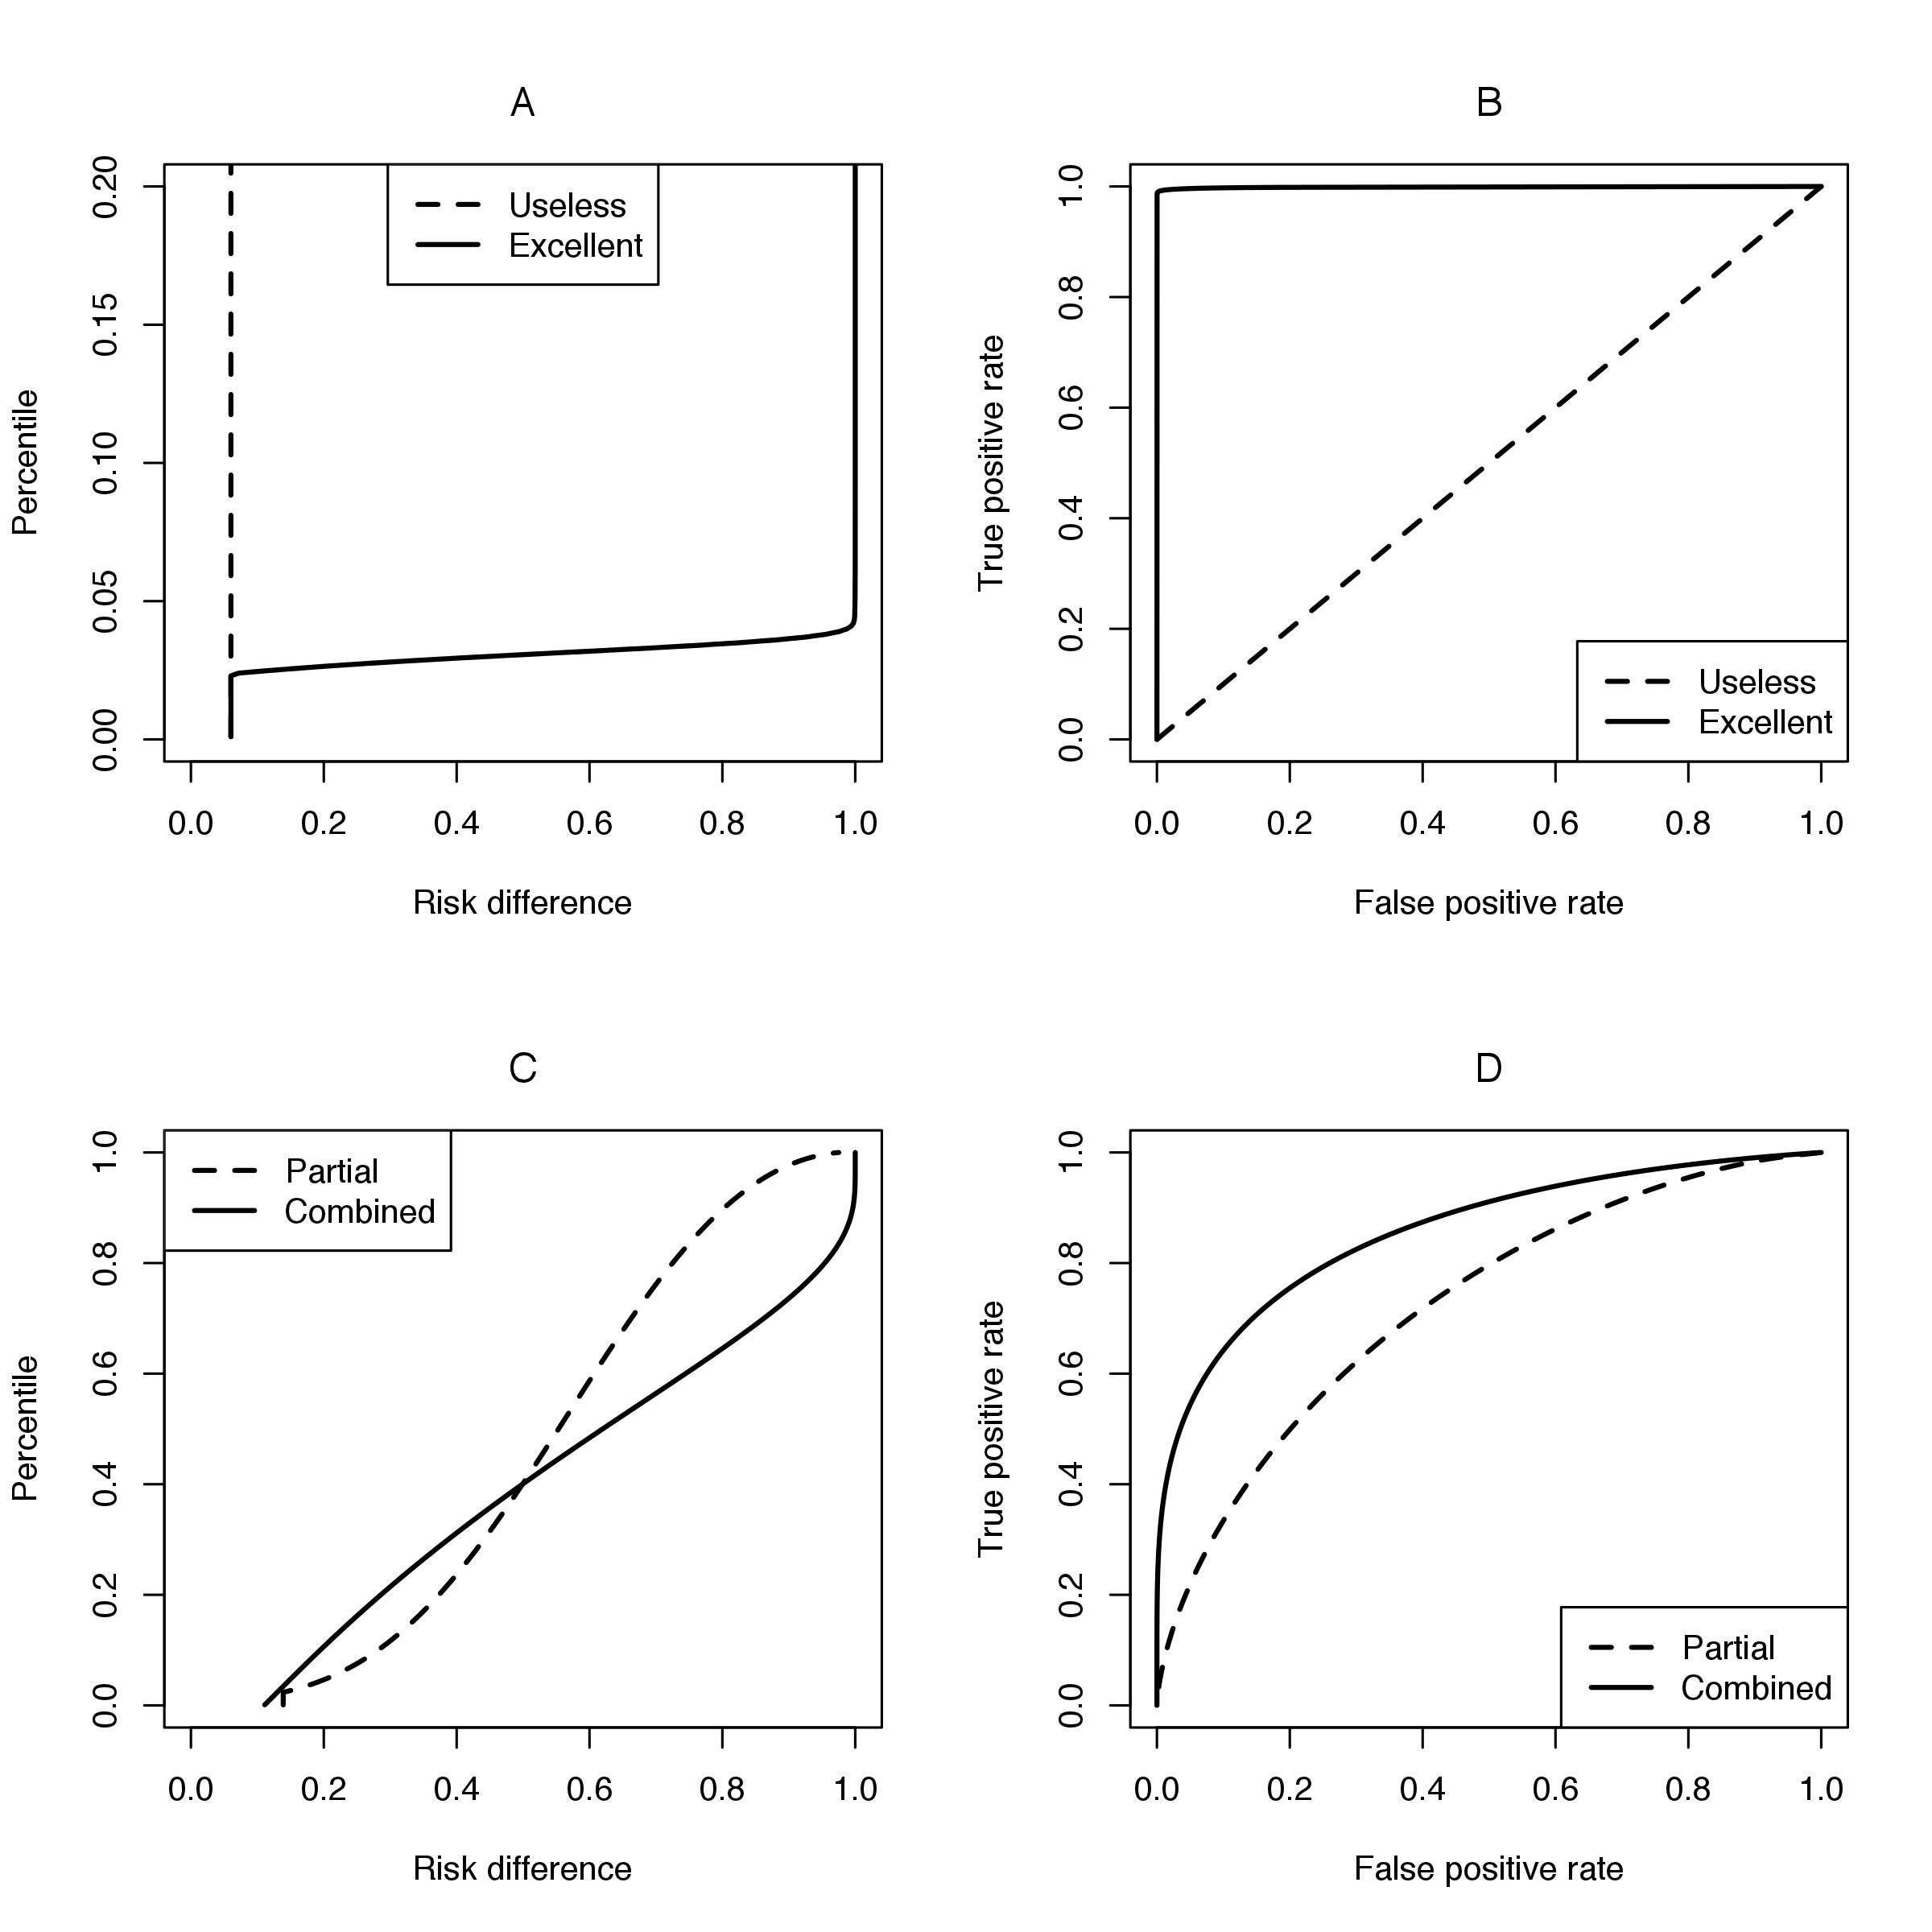
\includegraphics[scale=0.80]{Figure1.jpeg}
\end{center}
\caption{Panel A displays the CDF of the risk difference based on a useless and an ideal univariate surrogate. Panel B displays the ROC curves for the same ideal and useless surrogate candidates. Panel C displays the CDF of risk difference based on a medium quality univariate partial surrogate, and the CDF of risk difference based on a multivariate surrogate, which is the combination of two medium quality univariate partial surrogates. Panel D displays the ROC curves for the same medium quality univariate partial surrogate and multivariate surrogate. \label{4panel}}
\end{sidewaysfigure}

When A6 is observably violated the suggested estimators $FPF(t|c)$ and $TPF(t|c)$ are biased. However, under minor violations of A6 that might not be observable in the sample, the estimators are still reasonable estimates of useful quantities. Greater discussion of this point is given the Appendix A of the supplementary materials. When there are obvious violations of A6, the estimation of $FPF(t|c)$ and $TPF(t|c)$ should not be pursued. When Assumptions A6 is clearly violated we suggest the use of the $\widetilde{STG}$ and $CDF^{t}_{\Delta}(c)$ for comparison and evaluation or candidate surrogates.

\subsection{Cumulative Distribution Function of $\Delta$} \label{CDF}
 Let $CDF^{t}_{\Delta}(c)$ be the CDF of the risk difference $\Delta(t|S_{1,1}, \dots, S_{1,J})$, $CDF^{t}_{\Delta}(c)\equiv P\{\Delta(t|S_{1,1}, \dots, S_{1,J})\leq c\}.$ The $CDF^{t}_{\Delta}(c)$ versus $c$ curve is of interest for the evaluation of multivariate candidate PS and for the comparison of candidate PS. An ideal PS will have a $CDF^{t}_{\Delta}(c)$ versus $c$ plot that is a step function with a horizontal line at the proportion of subjects with $D(t)=-1$ and a horizontal line at the proportion of subjects with $D(t)=0$; where as defined previously $D(t)=Y^{t}(0)-Y^{t}(1)$. If we assume monotonicity of treatment effect, formally stated as
\begin{itemize}
\item A6: $T(z) \leq T(1-z)$ for one of the treatment arms $z$, $z=\{0,1\}$,
\end{itemize}
then the ideal PS candidate will have a $CDF^{t}_{\Delta}(c)$ versus $c$ plot with a single horizontal line at the proportion of subjects with $D(t)=0$ (in the case that A6 is $T(0) \leq T(1)$). If we alternatively assume no benefit, then the line will be at the proportion of subjects with $D(t)=-1$. Assumption A6 is not needed for the function $CDF^{t}_{\Delta}(c)$ to be well-defined. For a useless surrogate, the plot of $CDF^{t}_{\Delta}(c)$ versus $c$ will be a vertical line at $\rho_0(t)-\rho_1(t)$, the difference in prevalence of the potential clinical outcomes between the trial arms. Partially useful surrogates will have $CDF^{t}_{\Delta}(c)$ versus $c$ curves between these two curves with better surrogates having flatter curves. Figure \ref{4panel} displays the CDF of the risk difference for several different surrogate quality levels. We suggest the plug-in estimator of $\widehat{CDF}^{t}_{\Delta}(c)$, $\widehat{CDF}^{t}_{\Delta}(c)=\int{\mathrm{I}_{[\hat{\Delta}(t|s_{1,1,i}, \dots, s_{1,j,i})\leq c]} d\hat{F}_{S_1(1), \ldots, S_J(1)}(s_{1,1}, \dots, s_{1,J})}$. Although we display a useless surrogate in Figure \ref{4panel}, we suggest testing for any surrogate value prior to estimation of $\widehat{CDF}^{t}_{\Delta}(c)$ as it was found in simulations that there is evidence of bias when there is no variation in risk difference; a suggested test is given in Section \ref{CRE}.

Let $R^t(v)$ be the $v$th quantile of $\Delta(t|s_{1,1}, \dots, s_{1,J})$, where $R^t(v)=c$ for $v\in(0,1)$ such that $CDF^{t}_{\Delta}(c)=\{R^t\}^{-1}(v)$. The $R^t(v)$ versus $v$ curve has been called the predictiveness curve for the risk difference model. This curve has been previously suggested as a means of candidate PS comparison and evaluation \citep{Gilbert08}. The range of the curve is restricted by the range of risk difference, which is determined by the prevalence of the potential clinical events of interest in the population. Therefore, we prefer the $CDF^{t}_{\Delta}(c)$ versus $c$ curve for displaying the proportion of those subjects for which the treatment was ineffective at a given level of estimated risk difference. For characterization of the predictiveness of the model we prefer the classification accuracy measures.

\subsection{Time-dependent Standardized Total Gain} \label{STG}
It is easily shown that the area under the predictiveness curve, $R^t(v)$ versus $v$, is equal to $\rho_0(t)-\rho_1(t)$. For this reason, the area between the quantile curve $R^t(v)$ and the line $\rho_0(t)-\rho_1(t)$ on a plot against $v$ is of interest for evaluation and comparison of candidate PS. This area has been called the total gain (TG). \citet{Huang11} suggest a standardized version of TG for the comparison of PS for binary clinical endpoints. We extend the concept of total gain to the time-to-event setting and define the time-dependent total gain as $TG(t) = \int_0^{1}{|R^t(v) -(\rho_0(t) -\rho_1(t))|dv}$ and the time-dependent standardized total gain as $STG(t) \equiv TG(t)/[2(\rho_0(t) - \rho_1(t))\{1-\rho_0(t) + \rho_1(t)\}]$.

The $STG(t)$ is of interest for comparison of candidate surrogates regardless of the validity of assumption A6 as steeper quantile curves, and thus greater area between $R^t(v)$ and $(\rho_0(t) -\rho_1(t))$, correspond to better prediction of clinical treatment effect and a better candidate surrogate. Under A6, $STG(t)$ also has a useful interpretation based on the classification accuracy measures, given by $STG(t)=max_c\{\mbox{Sensitivity}(t|c) + \mbox{Specificity}(t|c)\} -1$. This interpretation follows directly from the proof given in \citet{Huang11} for the binary clinical endpoint setting. Given this interpretation, $STG(t)$ at a fixed time point is a useful single measurement for evaluation of univariate and multivariate candidate surrogates, as this is equivalent to the upper-most left point on the $ROC^{t}(q)$ curve for the same time point $t$.

We suggest plug-in estimators for $TG(t)$ and $STG(t)$ given by, 
\begin{eqnarray}
\widehat{TG}(t)&=&\int{|\widehat{\Delta}(t|s_{1,1}, \dots, s_{1,J}) -\{\hat{\rho}_0(t) -\hat{\rho}_1(t)\}|d\hat{F}_{S_1(1), \ldots, S_J(1)}(s_{1,1}, \dots, s_{1,J})} \hspace{4mm} \mbox{and} \label{TG} \\
\widehat{STG}(t)&=&\widehat{TG}(t)/[2(\hat{\rho}_0(t) - \hat{\rho}_1(t)]\{1-\hat{\rho}_0(t) + \hat{\rho}_1(t)\}.
\end{eqnarray}
Here $\{\hat{\rho}_0(t) -\hat{\rho}_1(t)\}$ is a maximum likelihood estimate. Even when assumption A6 does not hold, the difference in estimated $STG(t)$ can be used for inference to compare candidate PS in the same trial at a particular time point $t$, by Wald test of the null hypothesis $STG_1(t)-STG_2(t)=0$. 

As well, the same estimator we use at a fixed time point $t$ can be used to estimate the $STG(t)$ versus $t$ curve, for all $t$ greater than $\tau$ and less than the time of trial closure. This curve can be used to investigate time-variation in surrogate quality for a particular surrogate or for comparison. Curves, $STG(t)$ versus $t$, that have noticeable downward slopes may indicate that a candidate surrogate modifies the clinical treatment effect less over time, declining surrogate quality, or that the marginal risk difference is declining. To better understand the context of declining or increasing $STG(t)$ over time, the marginal risk differences over time should be graphed simultaneously. Figure \ref{STG} Panel A depicts a time-independent high quality surrogate and useless surrogate in a trial with declining marginal risk difference, Panel B depicts the same surrogates for a trial with increasing marginal risk difference. 

\subsection{Integrated Standardized Total Gain} \label{ISTG}
As an alternative to estimating the $STG$ at a fixed time $t$, we can summarize the $STG(t)$ by averaging over the estimated distribution of event times. We define the integrated $STG$ ($ISTG$) as $\int STG(t) \, dF(t)$, where $F(t)$ is the distribution function of the event times. The estimated marginal distribution of event times $\hat{F}(T)$ is calculated by integrating over $Z$ and $S$ in the conditional CDF defined by the assumption A5. Then the plug-in estimator of the integrated $STG$ is the expectation with respect to that distribution:
\[
 \widetilde{STG} = \int \widehat{STG}(t) \, d \hat{F}(t). 
\]
The $\widetilde{STG}$ can be used to summarize the surrogate quality without specifying a fixed time point. By borrowing information across times, it provides a useful, single value estimate for describing and comparing candidate surrogates. The $\widetilde{STG}$ difference between the candidate PS in the same trial can be used in the same way as the difference in $STG(t)$ for inference on comparison.

\subsection{Evaluation and Comparison of Candidate PS} \label{DEF}
Testing null hypothesis $H0_1$,  no surrogate value, using the biomarker associated coefficients from the risk estimation model as outlined in section \ref{CRE} is a first step in evaluation or comparing biomarkers as PS.  This test can also be used to help determine what biomarkers to include in a multivariate surrogate. One should first consider each biomarker as a univariate surrogate, eliminating those from consideration that are found to have no evidence of variation in the CEP-curve by $H0_1$. Then, combinations of the biomarkers can be considered as multivariate candidate surrogates, giving greater consideration to combinations of univariate candidates that were found to have some evidence of surrogate quality. The coefficient test of  null hypothesis $H0_1$ can again be used to reduce the dimension of multivariate surrogates, as a biomarker $j$ for which the coefficients $\gamma_{0j}=\gamma_{1j}=0$ in a multivariate surrogate can be considered to not add value to surrogate. Once the field of consideration has been narrowed to considered only candidates with at least some surrogate quality, PS can be further evaluated based on their $CDF^{t}_{\Delta}(c)$, $ROC^{t}(q)$ and the $STG(t)$ v $t$  curves. These curves can also help to give a visualization of a ranking of the candidates. 

The $STG(t)$ or $\widetilde{STG}$ difference between each of the candidates that are evaluated to have similarly high value as PS can be used to determine if there is statistical evidence to support the superiority of one of the candidates. The choice of time-point for comparison should be motivated by the scientific question of interest. For example, If one year treatment efficacy is of primary interest, a $t$ of one year less $\tau$ would be a logical choice from comparison. If there is no time point of particular scientific interest, inference should be based on $\widetilde{STG}$ difference and $CDF^{t}_{\Delta}(c)$, $ROC^{t}(q)$ should be considered at the longest follow-up time less $\tau$. As the CDF based risk is cumulative, a $t$ that is equal to the longest follow-up less $\tau$ includes all the available outcome information and allows for the best investigation of durability both of surrogacy and treatment effect. Comparisons over all observed follow-up times greater than $\tau$ can be investigated using the $STG(t)$ versus $t$ plots.

Ideally there will be a single candidate surrogate that has visually superior $CDF^{t}_{\Delta}(c)$, $ROC^{t}(q)$ that also has statistically significantly higher $\widetilde{STG}$ than all other candidates. This may not always be the case. When assumption A6 holds the candidate surrogate with the highest left-most point of the $ROC^{t}(q)$ curve should also be the candidate surrogate with the highest $STG(t)$. When A6 is violated this may not be true. When A6 does not hold, the candidate surrogate with the highest $\widetilde{STG}$ and a $CDF^{t}_{\Delta}(c)$ curve that is superior to all other candidates for at least some $c$, has the most value as a PS among the candidates considered. If this candidate is found to be statistically significantly superior to some or all the other candidates this provides greater evidence of superiority. However, as with almost all statistical tests, a failure to reject the null does not prove the null; lack of significant  $\widetilde{STG}$ difference does not prove lack of superiority.

\section{Simulation Studies}
Suppose the conditional CDF of $T$ given $S_j(1)$ and $Z$ follows a Weibull model and $\{S_j(1),W\}$ follows a multivariate truncated normal model with correlation R$_{S_jW}$ between each of the univariate candidates and the BIP and correlation R$_{S_kS_j}$ between each pair of candidates. Information lost to drop out occurs completely at random and at a rate of approximately 5\% per year. Event times are censored at 3 years after $\tau$, at which time the trials have 50\% cumulative treatment efficacy on average. An average of 103 treatment arm infections are observed by 3 years post $\tau$, corresponding to an annual incidence rate of 0.06, whereas an average of 206 control arm infections are observed in the same period, for an annual incidence rate of 0.12 over the 500 simulations. 

We investigate four different univariate candidate PSs with varying quality levels, a high quality surrogate with a $STG$ at year three, $STG(3)$, of 0.48, two marginal quality surrogates with $STG(3)$ of 0.1 and 0.24, and a null surrogate with $STG(t)=0$ for all time points $t$. We also investigate two scenarios where the true model for outcome contains a multivariate surrogate, where $S_1(1)$ and $S_2(1)$ combined under model A5 have a $STG(3)$ of 0.23 and 0.51, respectively. We investigate these different levels of candidate surrogates for two different BIP correlations, $R_{s_{1j}w}$, of 0.8 and 0.5. For the multivariate scenarios, we consider the correlation value sets ranging from $(R_{s_{1,1}w},R_{s_{1,2}w})\in\{(0.8,0.8), (0.5, 0.5)\}$ with a correlation between the candidate surrogates ranging from 0 to 0.3. Results for the 0.3 correlation are displayed. 500 replicates of the simulation were run for each scenario.  Some simulations did not converge and were removed from the simulations used for bias and power calculations; there was a 2.5\% non-convergence rate.  All candidate PS in the simulations are time invariant and therefore the characteristics of the $STG(t)$ estimator can be determined based on a single time-point $t$, for this we use the simulated trial terminal follow-up time of  3 years; results for time-dependent models can be found in Table 4, Appendix B of the supplementary materials. 

Bias results are displayed in Table \ref{Bias} and suggest that the semi-parametric EML method for the Weibull risk difference model is adequately unbiased and that the suggested estimators for $CDF^{t}_{\Delta}(c)$, $TPF(t|c)$, $FPF(t|c)$, $STG(t)$ and $\widetilde{STG}$ have adequate precision and accuracy in all cases for which they are applicable. As we have suggested above, there is some bias when there is no surrogate value. When there is no surrogate value the estimated model coefficients are still unbiased, with average bias less than 3\% of one Monte Carlo SD (results not displayed). The large standard deviation of the $STG(t)$ estimates over all the simulations may imply that this estimator is not as efficient as possible. A correlation of 0.5 or higher between a candidate PS and a BIP seems adequate for unbiased estimation of the suggested summary statistics and curves. The results for the joint Wald test of any surrogate value, displayed in Table \ref{Bias}, suggest that this test has correct Type 1 error and adequate power in all scenarios. Monte Carlo standard errors are used in all Wald tests due to the computational burden of the bootstrap.

Table \ref{Power} displays the power to discriminate between two surrogate quality levels based on the $STG(t)$ difference Wald test for fixed time point $t=3$. Monte Carlo standard errors are used and only those candidate surrogates with any surrogate quality are displayed. We find that for all null hypothesis scenarios the test has correct type 1 error. We also find that the test has adequate power to detect differences in $STG(3)$, particular when there is good correlation between the BIP and the candidate PS, with the power increasing with the difference in $STG(3)$, as expected. The test is not valid if either of the candidate surrogates has no surrogate value, as type 1 error is inflated when the true value is on the boundary of the parameter space (results not shown). 

Table \ref{Ipow} displays the power to discriminate between two surrogate quality levels based on the difference in integrated STG, $\widetilde{STG}$. We again find that for all null hypothesis scenarios the test has nearly a nominal 5\% Type 1 error rate with similar to slightly higher power than the $STG(3)$ difference test for the same scenarios. 

\begin{sidewaystable}[ht]
\begin{center}
\caption{Performance of Accuracy Measures and the Joint Wald Test of the Null Hypothesis of No Surrogate Value H0$_1$ \label{Bias}}
\begin{tabular}{lccccccc}
  \hline
&$R_{s_{1,j}w}^{**}$&$STG(3)=0$ & $STG(3)=0.1$  & $STG(3)=0.24$  & $STG(3)=0.48$&$STG(3)^{*}=0.23$&$STG(3)^{*}=0.51$\\ 
  \hline
Bias $CDF^{3}_{\Delta}(c)$& 0.8& 0.052 (0.009) & 0 (0.008) & 0.003 (0.009) & 0 (0.006) & 0 (0.009) & 0.006 (0.011) \\ 
 &0.5& 0.052 (0.009) & 0.001 (0.008) & 0.002 (0.009) & 0.002 (0.006) & -0.001 (0.009) & 0.025 (0.031) \\ 
Bias $TPF(3|c)$& 0.8& 0.544 (0.035) & 0.014 (0.058) & -0.024 (0.065) & 0.013 (0.048) & 0.063 (0.139) & 0.023 (0.037) \\ 
 &0.5& 0.56 (0.048) & 0.028 (0.07) & -0.006 (0.075) & 0.011 (0.047) & 0.062 (0.128) & 0.013 (0.072) \\ 
Bias $FPF(3|c)$& 0.8& 0.497 (0.002) & 0 (0.002) & 0.001 (0.003) & 0 (0.001) & -0.004 (0.01) & -0.004 (0.006) \\ 
 &0.5& 0.497 (0.002) & -0.001 (0.003) & 0 (0.003) & -0.001 (0.001) & -0.004 (0.009) & -0.012 (0.018) \\ 
Bias $STG(3)$& 0.8& 0.066 (0.053) & 0.021 (0.086) & -0.043 (0.101) & -0.004 (0.06) & 0.014 (0.064) & 0.047 (0.079) \\
  &0.5 & 0.09 (0.072) & 0.042 (0.103) & -0.016 (0.115) & -0.015 (0.059) & 0.025 (0.077) & 0.043 (0.158) \\ 
Bias $STG.i$ & 0.8 & 0.065 (0.079)& 0.021 (0.081)& 0.023 (0.051)& 0.003 (0.067) & 0.009 (0.075) & 0.041 (0.074) \\
 & 0.5 & 0.059 (0.099) & 0.052 (0.109) & 0.006 (0.053)& 0.007 (0.076)& 0.076 (0.224) & 0.024 (0.153) \\
\% Power H0$_1$& 0.8& 0.05 & 0.94 & 0.99 & 0.99 & 0.99 & 0.99 \\ 
  &0.5& 0.05 & 0.94 & 0.99 & 0.99 & 0.99 & 0.99 \\ 
   \hline
\multicolumn{8}{p{9in}}{Bias entries for the $TPF(3|c)$ and $FPF(3|c)$ curves are average bias over the simulations and 2000 points on each simulated curve (empirical standard deviation of the estimated statistic over the simulations). H0$_1$ is the null hypothesis of no surrogate value (i.e., no variation in risk difference over $S_j(1)$ for any time point), based on the joint Wald test of $\gamma_{0j}=\gamma_{1j}=0$ $\forall j\in\{1\ldots,J\}$. *Multivariate candidate PS, **For multivariate surrogate candidates $R_{s_{1,j}w}=x$ indicates the set $(R_{s_{1,1}w},R_{s_{1,2}w})=(x,x)$.}
\end{tabular}
\end{center}
\end{sidewaystable}

\begin{sidewaystable}[ht]
\begin{center}
\caption{Power of difference in $STG(t)$ tests for $t=3$ years \label{Power}}
\begin{tabular}{rrccccc}
  \hline
 & $R_{s_{1,j}w}$ & $STG(3)=0.1$  & $STG(3)=0.24$  & $STG(3)=0.48$& $STG(3)^{*}=0.23$  & $STG(3)^{*}=0.51$\\
  \hline
$STG(3)=0.1$ &0.5 & 4.80 & 15.80 & 80.40 & 16.90 & 58.20 \\ 
   &0.8 &7.20 & 31.20 & 90.00 & 32.80 & 96.40 \\ 
$STG(3)=0.24$ &0.5&  & 4.40 & 41.80 & 8.00 & 39.00 \\ 
   &0.8 &  & 5.20 & 49.60 & 10.00 & 69.60 \\ 
$STG(3)=0.48$&0.5 &  &  & 6.00 & 44.30 & 13.60 \\ 
   &0.8&  &  & 5.20 & 47.60 & 17.80 \\ 
$STG(3)^{*}=0.23$&(0.5, 0.5) &  &  &  & 3.80 & 21.60 \\ 
   &(0.8, 0.8) &  &  &  & 5.00 & 13.80 \\ 
$STG(3)^{*}=0.51$&(0.5, 0.5)&   &  &  &  & 2.40 \\ 
   &(0.8, 0.8)&  &  &  &  & 6.00 \\ 
   \hline
\multicolumn{7}{p{9in}}{Wald test for comparing two candidate surrogates by testing $STG_1(3)-STG_2(3)=0$. *Multivariate candidate PS, **For multivariate surrogate candidates $\rho_{s_{1,j}w}$ stands for $(R_{s_{1,1}w},R_{s_{1,2}w})$.}
\end{tabular}
\end{center}
\end{sidewaystable}

\begin{sidewaystable}[ht]
\begin{center}
\caption{Power of difference in $\widetilde{STG}$ tests for $t \in (\tau, 3.5)$ years \label{IPow}}
\begin{tabular}{rrccccc}
  \hline
 & $R_{s_{1,j}w}$ & $\widetilde{STG}=0.10$  & $\widetilde{STG}=0.25$  & $\widetilde{STG}=0.47$& $\widetilde{STG}^*=0.23$  & $\widetilde{STG}^*=0.52$\\
  \hline
$\widetilde{STG}=0.10$ & 0.8 & 4.8 & 14.4 & 75.6 & 24.6 & 56 \\ 
&  0.5  & 7.2 & 37.6 & 91.8 & 93.9 & 97.4 \\ 
 $\widetilde{STG}=0.25$ & 0.8 &  & 4 & 63.6 & 47.2 & 37.6 \\ 
&  0.5 &  & 4 & 78.8 & 80 & 94.8 \\ 
$\widetilde{STG}=0.47$ & 0.8 &  &  & 6 & 7.5 & 8.8 \\ 
 & 0.5 &  &  & 6 & 2.8 & 16.2 \\ 
$\widetilde{STG}^{*}=0.23$ & (0.8, 0.8) &  &  &  & 4.6 & 24.2 \\ 
&  (0.5, 0.5) &  &  &  & 6.3 & 17.2 \\ 
$\widetilde{STG}^{*}=0.52$ & (0.8, 0.8) &  &  &  &  & 1.6 \\ 
 & (0.5, 0.5) &  &  &  &  & 6 \\ 
   \hline
\multicolumn{7}{p{9in}}{Wald test for comparing two candidate surrogates by testing $\widetilde{STG}_1-\widetilde{STG}_2=0$. *Multivariate candidate PS, **For multivariate surrogate candidates $\rho_{s_{1,j}w}$ stands for $(R_{s_{1,1}w},R_{s_{1,2}w})$.}
\end{tabular}
\end{center}
\end{sidewaystable}


\section{Example}
The Diabetes Control and Complication Trial (DCCT) enrolled 1,441 persons with type 1 diabetes from 1983 to 1989 to determine the effects of intensive diabetes therapy on long-term complications of diabetes. Participants in the DCCT were randomly assigned to intensive diabetes therapy aimed at lowering glucose concentrations as close as safely possible to the normal range or to conventional therapy aimed at preventing hyperglycemic symptoms. One of the outcomes of the DCCT, nephropathy (damage to the kidneys), is the leading cause of death and dialysis in the young with type 1 diabetes, particularly those with poorly controlled glucose levels. Nephropathy is often defined by a high albumin excretion rate, as micro-albuminuria (defined as albumin excretion rate $>$ 30 mg/24 hr) is the least invasive gold standard for kidney damage. The trial ended early in 1993 due to strong evidence of treatment efficacy, with a longest follow-up time of 7.5 years after the biomarker measurments of interest; estimated adjusted mean risk of micro-albuminuria was reduced by 56\% (P-value 0.01)\citep{DCCT}. 

Although the trial could not be blinded to subjects or clinicians, it was blinded to investigators until the close of the trial. It is unlikely that the outcome would have been materially affected by subject or clinician knowledge of treatment status, as the only known risk factor in this population is poor diabetes management. Subjects that had dramatic behavioral changes while on trial were considered non-compliant and were censored at that point. This accounts for less than 3\% of person years in the trial and is balanced between treatment arms. The current analysis includes all participants who were free from micro-albuminuria at baseline (n = 1035); baseline micro-albuminuria is balanced over the arms of the trial. 

We consider four candidate surrogates: the difference in log-transformed hemoglobin A1C (HBA1C) measurements from baseline to year one, the difference in log-transformed estimated glomerular filtration rate (EGFR) measurements from baseline to year one, their linear combination into a univariate surrogate (HBA1C-EGFR) and the multivariate combination of the linear combination HBA1C-EGFR and HBA1C. Although there are some subjects for whom these values increased over the year, expert opinion is that increases were most likely due to measurement error or random fluctuation and are not indications of clinically relevant increases. We therefore truncate both candidate surrogates at zero for our primary analysis. EGFR values increased in only 1.2\% of subjects, 6.1\% for HBA1C and both increased in only one subject. This is consistent with the error for both being random. As a sensitivity analysis, we repeat the analysis with the non-truncated measurements and found the the results were similar, no reported. 

The event of interest is the onset of persistent micro-albuminuria, which is defined as having two consecutive albumin excretion rate measurements $>$ 30 mg/g. No subjects had an event prior to 1 year post-randomization. All subjects had the BIPs measured, which is defined as a linear combination of baseline laboratory measurements and demographic variables. The estimated linear correlation between the joint linear combination BIP and the candidate PS are 0.57 and 0.76 for HBA1C and univariate linear combination HBA1C-EGFR, respectively. All three univariate candidate PS also have respective individual BIPs. The correlation between the individual BIP and their PS are 0.7, for HBA1C, 0.88 for EGFR and 0.76 for the univariate linear combination HBA1C-EGFR. The individual BIPs are used for investigation of each biomarkers' univariate PS value, as well as comparison between the three univariate PS candidates. The joint linear combination BIP is used for the combined model. For all analyses we fit the conditional Weibull model proposed in A5 via the semi-parametric EML method and perform 1000 bootstraps. 

The analysis indicates that HBA1C has clear surrogate value, with P-value for testing H0$_1$ of 0.001. The P-value for testing H0$_1$ for EGFR is 0.19. The univariate linear combination HBA1C-EGFR has a P-value for testing H0$_1$ of 0.055. The multivariate candidate PS of HBA1C combined with the univariate linear combination HBA1C-EGFR has an estimated P-value for testing H0$_1$ of 0.018. Based on the tests of H0$_1$ alone there is some evidence that HBA1C and both the combination candidate surrogates are better than EGFR alone. The estimated $\widehat{\widetilde{STG}}$ is 0.2 for HBA1C alone and 0.15 for the univariate linear combination HBA1C-EGFR; their multivariate combination has a $\widehat{\widetilde{STG}}$ of 0.202. Given that there is no evidence to suggest that EGFR alone has any value as a PS, we do not pursue estimation or testing of any of the suggested summary statistics.

The P-value for the test that $\widehat{\widetilde{STG}}$ difference between HBA1C alone and the univariate the linear combination of HBA1C-EGFR is zero, is 0.057. This is evidence that HBA1C alone is superior to the univariate the linear combination of HBA1C-EGFR. As the difference between $\widehat{\widetilde{STG}}$ for HBA1C alone and the multivariate candidate PS is so small, it is not surprising that the P-value for the null that their difference is equal to zero is 0.99. 

Figure \ref{exp} Panel A depicts the $\widehat{CDF}^{7.5}(c)$ versus $c$ curves for all four candidate surrogates, HBA1C, EGFR the univariate linear combination HBA1C-EGFR and the multivariate combination. The EGFR curve is most similar to the marginal risk difference line, supporting the finding that EGFR has little value as a PS. The multivariate combination surrogate which is flatter than the EGFR alone curve is very similar to HBA1C curve. This provides further evidence that the combination candidate does not improve upon HBA1C alone. We use time-point year 7.5 for our main analysis because it is the longest follow-up time in the trial. As there is no evidence of violation of A6, Figure \ref{exp} Panel B displays the $\widehat{ROC}^{7.5}(q)$ versus $q$ curves for the HBA1C and the two combination candidates. Figure \ref{exp} Panel C depicts the $STG(t)$ versus $t$ for $t$ greater than one year for HBA1C and the two combination candidates. Both Panels B and C support that there is no significant difference between HBA1C alone and the multivariate combination, but that HBA1C alone is significantly better than the univariate linear combination candidate.

A naive evaluation of the association of the two univariate candidate surrogates and outcome separately in each arm
of the trial, using a Cox proportional hazards model and the hazard ratio magnitude for ranking, gives the same ranking of candidate surrogates in the treatment arm as do our methods. The findings support our conclusion that EGFR has no association with outcome under treatment. However, in the control arm EGFR is significantly associated with outcome and HBA1C is not. Although the naive analyses finds some evidence that HBA1C is a better candidate surrogate than EGFR under treatment, it will not always be the case that rank is preserved among the correlates of risk in the treatment arm alone. The surrogate evaluation literature has many examples of biomarkers that are highly correlated with outcome under treatment alone, but are not associated with treatment efficacy \citep{flemming96}.  

\begin{sidewaysfigure}[H]
\begin{center}
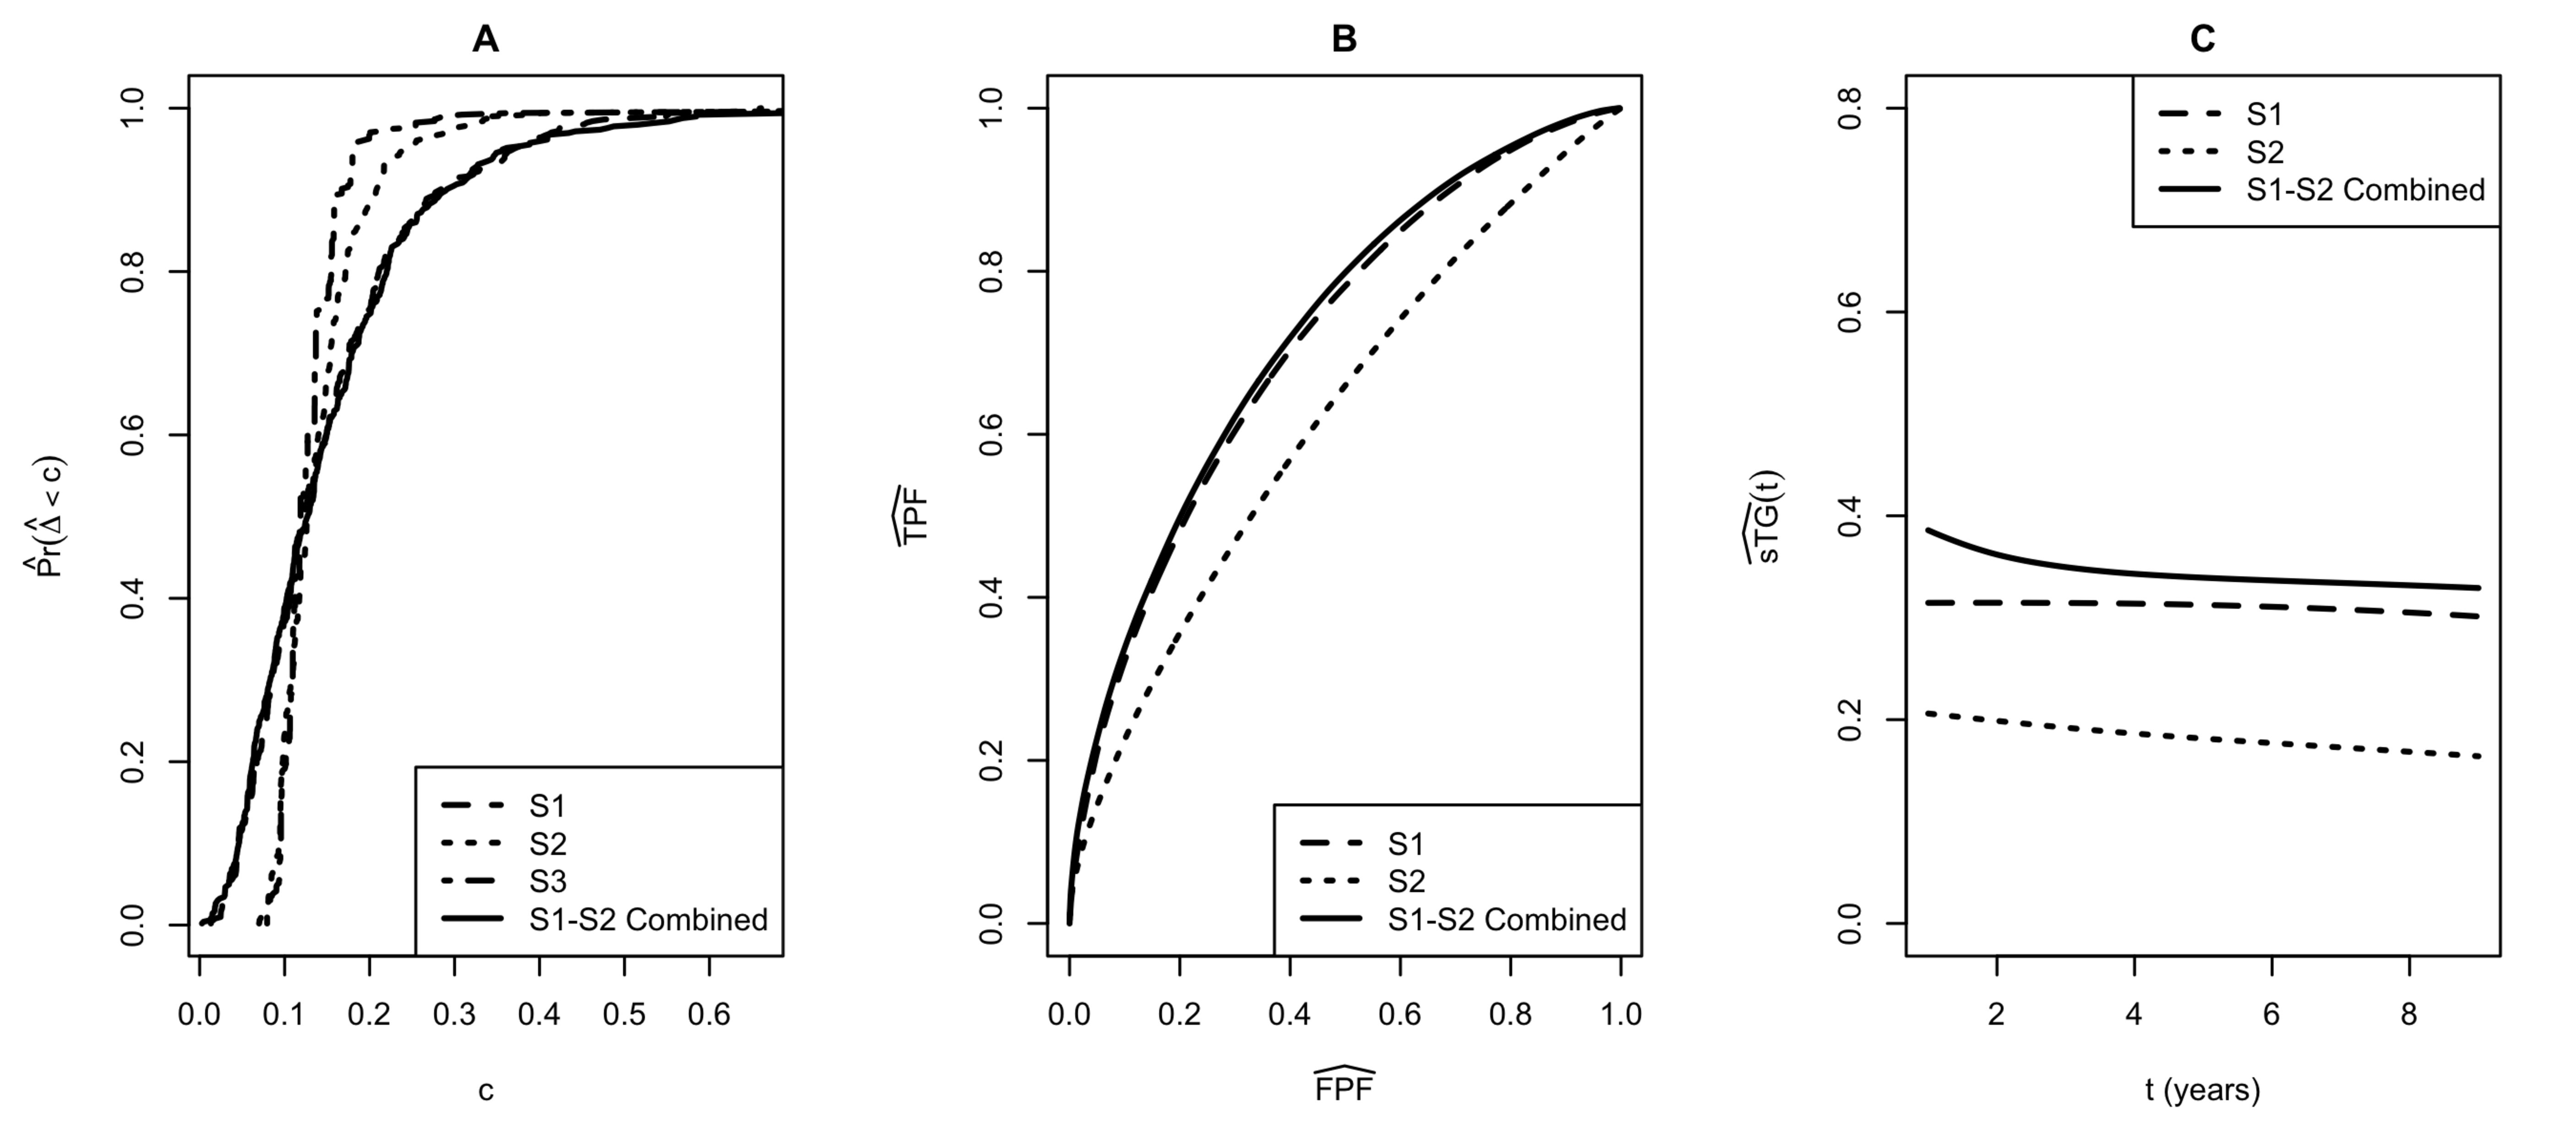
\includegraphics[scale=0.65]{dcct-example-figure-2014-6-2.pdf}
\end{center}
\caption{Panel A depicts the estimated $CDF^{8.5}(c)$ versus $c$ for the truncated univariate candidate principal surrogates HBA1C and EGFR as well as for the univariate linear combination HBA1C-EGFR candidate and the multivariate candidate PS. Panel B depicts the estimated $ROC^{8.5}(q)$ versus $q$ for HBA1C and both of the combination candidate. Both panels suggest that HBA1C is better than EGFR alone or their univariate combination and that there is no significant difference between multivariate combination and HBA1C alone. Panel C depicts the $STG(t)$ versus $t$ for each of truncated candidate PS that showed some evidence of surrogate value, HBA1C and the univariate combination HBA1C-EGFR and the multivariate combination, for $t$ greater than one year and less than the trial close of nine years. \label{exp}}
\end{sidewaysfigure}

\section{Discussion}
Principal surrogates are important endpoints for Phase I and II trials. Without reliable surrogate endpoints for these trials, treatment development is slowed, allowing poor treatments to be advanced to Phase III and abandoning potentially effective formulations prior to Phase III. Few PS evaluation methods allow for comparison of candidate PS or for the evaluation of combinations of biomarkers as candidate PS and the few existing methods for comparison or combination of biomarkers as candidate PS have not been explored for time-to-event data. Our proposed Weibull model extension of the \citet{Huang11} semi-parametric EML method as well as our proposed classification accuracy and summary measures accommodate evaluation of multivariate PS and comparison of candidate PS using time-to-event data. 

Although our proposed estimands and estimators for the classification accuracy curves depend on assumption A6 to be well-defined, we show that when there are small undetectable violations of A6, the estimates approximate the desirable modified estimands of no-benefit or unaffected ROC curves (Appendix A supplementary materials). Even when A6 is clearly violated, the suggested $CDF^{t}_{\Delta}(c)$ and $STG(t)$ versus $t$ curves allow for visual comparison of candidate surrogates and the $STG(t)$ or $\widetilde{STG}$ difference tests perform well for discriminating between two candidate PS that both have some value as a PS. While only the risk estimands themselves and the proposed $CDF^{t}(c)$ curve perform well for biomarkers with no surrogate value, our proposed coefficient-based test of any surrogate value has satisfactory power and correct Type 1 error rate. Using the proposed methods we were able to show that the DCCT candidate surrogate HBA1C has more value as a PS than EGFR, and that the combination of HBA1C and EGFR in the same risk model was not an improvement over HBA1C alone.

Our proposed semi-parametric EML estimators seem to perform well when there is a predictive BIP with correlation with the candidate PS of at least 0.5. The performance decreases with the correlation of the BIP and $S_j(1)$, as has been illustrated for previous EML methods. This is a limitation of EML based methods, however, for the motivating example the BIP correlation exceeds $0.5$. The need for a joint BIP that is well correlated with all biomarkers included in a multivariate PS model is also a limitation of the methods. Methods allowing for the use of individual BIP for each biomarker included in a multivariate PS model would be a useful extension to our methods. Although it is not the focus of this work, our model allows for time-variation in the hazard, an extension to the existing time-to-event PS evaluation methods \citep{Qin07, Miao13}. This extension is discussed in greater detail in the supplementary materials where we consider a more complex Weibull model allowing for time-variation in the treatment effect and the surrogate quality following \citet{Gabriel13}.



\bibliographystyle{statmed}
%\bibliographystyle{unsrtnat}
\bibliography{bib_dissertation}
\end{document}




